%!TEX root = ../template.tex
%%%%%%%%%%%%%%%%%%%%%%%%%%%%%%%%%%%%%%%%%%%%%%%%%%%%%%%%%%%%%%%%%%%%
%% chapter3.tex
%% NOVA thesis document file
%%
%% This chapter includes a Literary Review.
%%%%%%%%%%%%%%%%%%%%%%%%%%%%%%%%%%%%%%%%%%%%%%%%%%%%%%%%%%%%%%%%%%%%
\chapter{Literature Review}
\label{cha:literature_review}

In this chapter, I provide a literary review on the three most important
subjects for the work of this thesis: \gls{AP}, tomographic algorithms
and \gls{DOAS} tomography instrumentation.

\section{Air pollution and pollutants}%
\label{sec:air_pollution_and_pollutants}

As stated in Section~\ref{sec:research_question}, the definition of
\gls{AP} is dependent on the context. Here, I will focus especially on
the effects of pollutants on human health. Whether these effects are the
most significant problems stemming from \gls{AP} is debatable (climate
change is mostly caused by anthropogenic production of greenhouse gases,
which are pollutants) but for this system and its intended uses, health
effects are definitely more prominent. Human health implications of a
polluted atmosphere are documented in very numerous studies throughout
the literature. In this document, I will only present a small number of
representative reviews and reports.

In 2004, \gls{WHO} published a report summarizing what was then the most
recent information on health effects of air pollution over Europe. This
review concluded that, even with all the regulations on \gls{AP} put in
place by the European authorities, its levels were still posed a
considerable burden on health throughout
Europe~\cite{WorldHealthOrganisationEurope2004}.

Although there are several hundred potentially harmful components
already that have already been found in the atmosphere, this report
addresses only \gls{PM}, ground level Ozone and Nitrogen Dioxide. As
many other studies had found, this Systematic Literature Review
(\gls{SLR}) identified several short-term and long-term exposure effects
for the three pollutants. The study found that short-term exposure to
all three substances were responsible for an increase in mortality and
hospital admissions, and that both \gls{PM} and O$_3$ increased the
population's usage of medication. Long-term exposure to all three
components have adverse pulmonary effects, but \gls{PM} have many other
negative effects. The most important of them a reduction in life
expectancy, which the authors attribute to cardiopulmonary mortality and
lung cancer.

Particulate Matter are described as airborne solid particles or
droplets. These particles vary in size, origin and composition, however,
it is usual to classify them by size, since that is what governs
particle deposition in the respiratory system. Urban \gls{PM} are
usually divided into three categories: coarse, fine and ultrafine.
Convention dictates that coarse particles have an aerodynamic diameter
of less that 10$\mu$m (PM$_{10}$), fine particles less than 2.5$\mu$m
(PM$_{2.5}$). In this review, the authors stated that the role that
ultrafine particles play in human health is still undetermined, but they
noted that coarse and (especially) fine particles are highly correlated
with an increase in mortality and the prevalence of respiratory
syndromes~\cite{WorldHealthOrganisationEurope2004}. 

Ground-level ozone is produced as a result of a chemical reaction
between nitrous oxides and Volatile Organic Compounds (\gls{VOC}), which
can be emitted either by natural source or by human-related activities.
O$_3$ is a powerful oxidant, and can easily accept electrons from other
molecules. In the respiratory tract, this chemical destroys double bonds
of the fatty acids in the surface of its lining. The process leads to
the deposition of several substances like aldehydes and hydrogen
peroxide, resulting in impaired cell function. Ozone is toxic at
concentrations that occur in urban areas around the world. On a more
ecological level, it has been established that O$_3$ is responsible for
a decrease in the trees' capabilities to assimilate carbon, which can
result in deforestation\todo{citations}.

Nitrous Oxides originate from the use of Internal Combustion Engines
(\gls{ICE}) for energy production and especially movement. It is usually
used as an indicator for the presence of heavy traffic. The compound
acts in a more subtle way than Ozone, described above. It increases the
risk of respiratory infections and can cause pulmonary edema. Moreover,
it has an effect on the immunological system, impairing the ability of
T-lymphocytes to address microbiological threats like viruses. Nitrous
oxides are also known to affect weaker populations, like children and
the elderly.







\section{Tomographic algorithms and reconstruction techniques}%
\label{sec:tomographic_algorithms_and_reconstruction_techniques}

\subsection{Introduction}%
\label{sub:introduction}

Tomography is the cross-sectional imaging of an object through the use
of transmitted or reflected waves, captured by the object exposure to
the waves from a set of known angles. It has many different applications
in science, industry, and most prominently, medicine. Since the
invention of the Computed Tomography (\gls{CT}) machine in 1972, by
Hounsfielf~\cite{Gunderman2006}, tomographic imaging techniques have had
a revolutionary impact, allowing doctors to see inside their patients,
without having to subject them to more invasive
procedures~\cite{Kak2001}.

Mathematical basis for tomography were set by Johannes Radon in 1917. At
the time, he postulated that  it is possible to represent a function
written in $\mathbb{R}$ in the space of straight lines, $\mathbb{L}$
through the function's line integrals. A line integral is an integral in
which the function that is being integrated is evaluated along a curved
path, a line. In the tomographic case, these line integrals represent a
measurement on a ray that traverses the Region Of Interest (\gls{ROI}).
Each set of line integrals, characterized by an incidence angle, is
called a projection (see Figure~\ref{fig:projection}). To perform a
tomographic reconstruction, the machine must take many projections
around the object. To the set of projections arranged in matrix form by
detector and projection angle, we call sinogram. All reconstruction
methods, analytical and iterative, revolve around going from reality to
sinogram to image~\cite{Bruyant2002, Kak2001, Herman1973, Herman1995,
Herman2009, Defrise2003}.

\begin{figure}[htpb]
    \centering
    \missingfigure{Projection Schematic}
    \caption{A schematic representation of a projection.}
    \label{fig:projection}
\end{figure}

There are two broad algorithm families when it comes to tomographic
reconstruction, regarding the physics of the problem. The problem can
involve either non-diffracting sources (light travels in straight
lines), such as the X-Rays in a conventional \gls{CT} exam; or
diffracting sources, such as micro-waves or ultrasound in more
research-oriented applications. In this document, I will not address the
latter family, since I will not be applying them in my work. In the next
few paragraphs, I will discuss the first family of algorithms, and
describe how an image can be reconstructed from an object's projections
when the radiation source is non-diffracting.

Let's consider the case in which we deal with a single ray of solar
light entering the atmosphere at a given point. Since the atmosphere
contains numerous absorbents and comparable atmospheric effects, the ray
changes from the point where it enters the atmosphere to the point at
which it is measured by a detector. Total absorption will depend on the
pollutant species, their cross-section and their concentration, since it
obeys Lambert-Beer's law. Looking from another angle, this absorption
is also the line integral that we will use to reconstruct our image.
With \gls{DOAS}, it is possible to measure several pollutants at the
same time, but for simplicity (and since it is one of the most studied
compounds in the field), let's consider that the single pollutant in our
atmospheric mixture is NO$_2$.

\subsection{Initial Considerations}%
\label{sub:initial_considerations}


The problem of tomographic reconstruction can be approached in a number
of ways, depending mostly on the authors. In my literary search, I have
found that Kak and Slaney~\cite{Kak2001} have certainly explained this
problem in one of the clearer ways available. Therefore, I shall base
the rest of my presentation in their writings, and complement with other
authors' notes wherever necessary.

Considering the coordinate system displayed in
Figure~\ref{fig:coordinates}. In this schematic, the object is
represented by the function $f(x, y)$. The  $(\theta, t)$ parameters can
be used to define any line in this schematic. Line AB in particular can
be written:

\begin{equation}
    \label{eq:lineAB}
    x \cdot \cos(\theta) + y \cdot \sin(\theta) = t
\end{equation}

\begin{figure}[htpb]
    \centering
    \missingfigure{Coordinates system}
    \caption{Schematic representation for coordinate setting.}
    \label{fig:coordinates}
\end{figure}

And if we were to write a line integral along this line, it would look
like Equation~\ref{eq:lineABIntegral}, the Radon transform of function
$f(x, y)$:

\begin{equation}
    \label{eq:lineABIntegral}
    P_{\theta}(t) = \int_{-\infty}^{\infty} f(x, y) \cdot \delta(x \cdot
    \cos(\theta) + y \cdot \sin(\theta) - t) dxdy
\end{equation}

Where $\delta$, the delta function, is defined in
Equation~\ref{eq:delta}.

\begin{equation}
    \label{eq:delta}
    \delta (\phi) =  
    \begin{cases}
            1, & \phi = 0\\
            0, & otherwise
    \end{cases}
\end{equation}

As I have mentioned previously, a projection is a set of line integrals
such as $P_{\theta}(t)$. Geometry plays a very important role in how the
integrals are written and solved for reconstruction. The simplest case
is the one where the set is acquired in a row, describing what is called
a parallel geometry. Another more complex case is when a single point
source is used as origin for all rays, forming a fan. This is called a
fanbeam array. There are other possible geometries, but they fall out of
the scope of this work and will therefore not be addressed any further.

\subsection{The Fourier Slice Theorem}%
\label{sub:the_fourier_slice_theorem}

The Fourier Slice Theorem (\gls{FST}) is the most important component of
the most important algorithm in tomographic inversion, the Filtered
BackProjection algorithm (\gls{FBP}). \gls{FST} is based on the equality
relation between the 
two-dimensional Fourier Transform (\gls{FT}) of the object function and
the one-dimensional \gls{FT} of the object's projection at an angle
$\theta$. Let's start by writing the 2D \gls{FT} for the object
function, Equation~\ref{eq:objectFT}, and the 1D \gls{FT} of projection
P$_\theta$, in Equation~\ref{eq:1dFTproj}.

\begin{equation}
    \label{eq:objectFT}
    F(u, v) = \int_{-\infty}^{\infty} \int_{-\infty}^{\infty} f(x, y)
    \cdot \exp \left [ -j2\pi (ux + vy) \right ] dx dy 
\end{equation}

\begin{equation}
    \label{eq:1dFTproj}
    S_{\theta}(\omega) = \int_{-\infty}^{\infty} P_{\theta} \cdot \exp\left[
    -j2 \pi \omega t \right]
\end{equation}

For simplicity, let's consider the 2D \gls{FT} at the line defined by
$v=0$ in the frequency domain. We rewrite the 2D \gls{FT} integral as:

\begin{equation}
    \label{eq:v0}
    F(u, 0) = \int_{-\infty}^{\infty} \int_{-\infty}^{\infty} f(x, y)
    \cdot \exp \left[  -j 2\pi  \omega ux \right] dx dy
\end{equation}

Notice that $y$ is not present in the phase factor of the \gls{FT}
expression anymore, and this means we can rearrange the integral as:

\begin{equation}
    \label{eq:v02}
    F(u, 0) = \int_{-\infty}^{\infty} \left[ \mathbf{\int_{-\infty}^{\infty}
    f(x, y) dy }\right] \cdot \exp \left[  -j 2\pi  \omega ux \right] dx 
\end{equation}

Now, the \textbf{bold} part of Equation~\ref{eq:v02} is similar to
Equation~\ref{eq:lineABIntegral}. It is precisely that equation,
considering $\theta=0$ and a constant value of $x$, as in
Equation~\ref{eq:p0}.

\begin{equation}
    \label{eq:p0}
    P_{\theta=0} (x) = \int_{-\infty}^{\infty} f(x, y) dy
\end{equation}

This in turn can be substituted in Equation~\ref{eq:v02}, finally
arriving at:

\begin{equation}
    \label{eq:FTP}
    F(u, 0) = \int_{-\infty}^{\infty} P_{\theta=0} (x) \cdot \exp \left[
    -j 2\pi ux \right] dx
\end{equation}

And this is the one-dimensional \gls{FT} for the projection at angle
$\theta=0$. Finally, the enunciation of the Fourier Slice Theorem:
\begin{center}
    \begin{minipage}{0.8\textwidth}

        \noindent\textbf{\emph{The Fourier Transform of a parallel
                projection  of an image $f(x, y)$ taken at angle
                $\theta$ gives a slice of the two-dimensional Fourier
                Transform, $F(u, v)$, subtending an angle $\theta$ with
                the $u$-axis (see Figure~\ref{fig:fst})}}

    \end{minipage}
\end{center}

\begin{figure}[htpb]
    \centering
    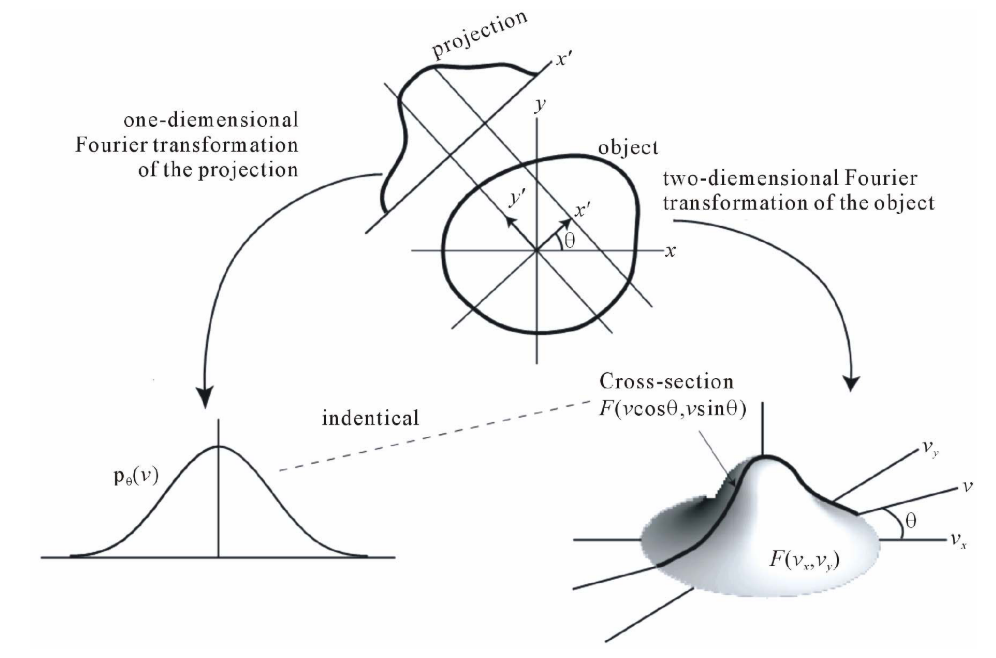
\includegraphics[width =.8\textwidth]{img/fst.png}    
    \caption{The \gls{FST}, a schematic representation.}
    \label{fig:fst}
\end{figure}

\subsection{The Filtered BackProjection Algorithm}%
\label{sub:the_filtered_backprojection_algorithm}

\subsubsection{The rationale for \gls{FBP}}%
\label{ssub:the_rationale_for_fbp}

If one takes the \gls{FST} into account, the idea behind the \gls{FBP}
seems to appear almost naturally. Say one has a single projection and
its Fourier transform. From the \gls{FST}, this projection is the same
as the object's two-dimensional \gls{FT} in a single line. A crude
reconstruction of the original object would result if someone were to
place this projection in its right place in the Fourier domain and then
perform a two-dimensional \gls{IFT}, while assuming every other
projection to be 0. The result, in the image space, would be as if
someone had smeared the object in the projections direction.

What is really needed for a correct reconstruction is to do this many
times, with many projections. This brings a problem with the method:
smearing the object in all directions will clearly produce a wrong
\emph{accumulation} in the center of the image, since every projection
passes through the middle (remember we are still talking about parallel
geometry projections) and are summed on top of each other, but on the
outer edges, this does not occur. If one does not address this, the
image intensity levels in the reconstructed image will be severely
overestimated in the center and underestimated in the edges (due to
normalization). The solution is conceptually easy: we multiply the
Fourier transform by a weighting filter proportional to its frequency
($\omega$) and that encompasses its relevance in the global scheme of
projections. If there are $K$ projections, then it is adequate for this
value to be $\frac{2\pi\lvert\omega\rvert}{K}$. As an algorithm,
\gls{FBP} can be written as in Algorithm~\ref{alg:fbp}.

\begin{algorithm}
    \caption{The Filtered BackProjection Algorithm}
    \label{alg:fbp}
    \begin{algorithmic}
        \FORALL{$\theta, \theta \in \left\{0..180,
        \frac{180}{K}\right\}$}
        \STATE{Measure projection $P_{\theta}(t)$;}
        \STATE{FT($P_{\theta}(t)$), rendering $S_{\theta}(\omega)$}
        \STATE{Multiply by $\frac{2\pi\lvert{\omega}\rvert}{K}$;}
        \STATE{Sum the \gls{IFT} of the result in the image space.}
    \ENDFOR
    \end{algorithmic}
\end{algorithm}

\subsubsection{Fan Projections Reconstruction}%
\label{ssub:fan_projections_reconstruction}

Parallel projections, in which the object is scanned linearly from
multiple directions, have the advantage of having a relatively simple
reconstruction scheme. However, they usually result in acquisition times
which are in the order of minutes. A faster way of collecting the data
is one where all radiation emanates from a single point-source, which
rotates around the target object (as well as the detectors). There are
two types of fan beam projections: equiangular and equally spaced. In
this project, I have only worked with equiangular processes, so I will
not include an explanation for equally spaced fan beam projections. The
reader may find this well described (much better than I would be able
to) in ~\cite{Kak2001} and ~\cite{Herman1973}.

Consider Figure~\ref{fig:equiangular}. If our projection data were
acquired through a parallel ray geometry, we would be able to say that
ray SA belonged to a projection $P_{\theta}(t)$, in which $\theta$ and
$t$ would be written:

\begin{equation}
    \label{eq:theta_and_t}
    \theta = \beta + \gamma \quad \text{ and } \quad t = D \cdot \sin \gamma
\end{equation}

In Equation~\ref{eq:theta_and_t}, $D$ is the distance between the source
$S$ and the origin $O$; $\gamma$ is the angle of a ray within a fan and
$\beta$ is the angle that the source $S$ makes with a reference axis.

\begin{figure}[htpb]
    \centering
    \missingfigure{kak and slaney fig 3.19}
    \caption{Schematic representation of an equiangular fan beam
    projection.}
    \label{fig:equiangular}
\end{figure}

%##doas
\section{DOAS}%
\label{sec:doas}

Differential Optical Absorption Spectroscopy is a well-established
absorption technique that is widely used in the field of atmospheric
studies~\cite{Platt2007}. There are two main families of \gls{DOAS}
assemblies, with different goals and capabilities:
\begin{itemize}

        \item Active systems, of which a simple illustration is
            presented in Fig.~\ref{fig:activeSmall}, are characterized
            by relying on an artificial light source for their
            measurements. A spectrometer at the end of the light path
            performs spectroscopic detection. Active DOAS techniques are
            very similar to traditional in-lab absorption spectroscopy
            techniques \cite{Platt2007};

        \item Passive DOAS techniques, illustrated in
            Fig.~\ref{fig:passiveSchematic}, use natural light sources,
            such as the Sun and the moon, in their measurement process.
            An optical system is pointed in certain elevation and
            azimuth angles and sends the captured light into a
            spectrometer, connected to a computer. The system returns
            the total value of the light absorption in its
            path~\cite{Platt2007,Merlaud2013}.

\end{itemize}

%f2
 \begin{figure*}[t]
    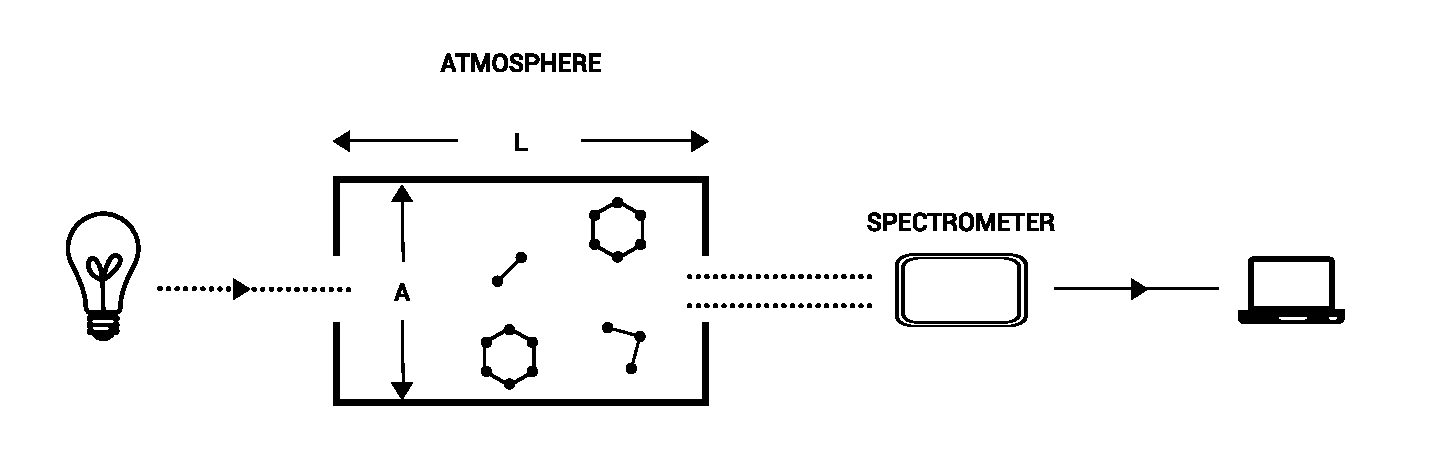
\includegraphics[width=14cm]{img/amt-2016-314-f02.pdf}
    \caption{Active DOAS schematic.}\label{fig:activeSmall}
  \end{figure*}

%f3
  \begin{figure*}[t]
      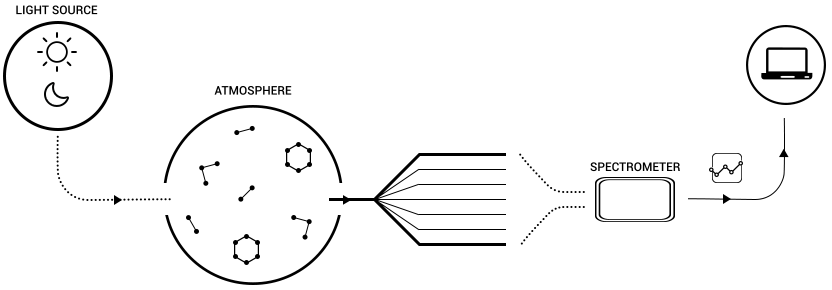
\includegraphics[width=14cm]{img/amt-2016-314-f03.png}
      \caption{Passive DOAS schematic.}\label{fig:passiveSchematic}
  \end{figure*}

DOAS itself is based on Lambert--Beer's law, which can be written as
\cite{Platt2007}

\begin{equation}
  \centering
  \label{eq:lambertBeer}
  I(\lambda) = I_0 (\lambda) \cdot \exp(-\sigma(\lambda) \cdot c \cdot L) \;,
\end{equation}

Where $\lambda$ is the wavelength of the emitted light; $I(\lambda)$ is
the light intensity as measured by the system; $I_{0}(\lambda)$ is the
intensity of the light as emitted by the source; and $\sigma(\lambda)$
is the absorption cross section of absorber, which is wavelength
dependent; $c$ is the concentration of the absorber we want to measure.


This law allows the definition of optical thickness
($\tau$)~\cite{Platt2007}:

\begin{equation}
      \label{eq:opticalThickness}
      \tau(\lambda) = \ln \bigg( \frac{I_{0}(\lambda)}{I(\lambda)}\bigg) = \sigma(\lambda) \cdot c \cdot
      L.
\end{equation}

In a laboratory setting, Eq.~(\ref{eq:lambertBeer})
or~(\ref{eq:opticalThickness}) can be used to directly calculate an
absorber's concentration, provided there is knowledge of  its cross
section. In the open atmosphere, however, absorption spectroscopy
techniques are far more complex. On one hand, $I_0(\lambda)$ is not
accessible since we measure from inside the medium we want to measure.
On the other hand, there are several environmental and instrumental
effects that influence measurement results. These effects include the
following~\cite{Platt2007}.

\begin{itemize}
      \item Rayleigh scattering is due to small molecules present in the
          atmosphere and is heavily influenced by wavelength (hence the
          blue colour of the
      sky).
      \item Mie scattering is caused by particles and larger molecules
          suspended in the atmosphere and is not very dependent
      on the wavelength (hence the white colour of clouds).
      \item Instrumental and turbulence effects are the instrument's
          transmissivity and atmospheric turbulence in the optical path
          also limit light intensity.

  \end{itemize}

In addition, we also have to take into account that, in the atmosphere,
there are a number of trace gases that interfere with passing light.

Another aspect worth mentioning is that our device is never pointed
directly at the light source (the Sun) but always processes light that
has been scattered at some unknown point in the optical path. This means
that the light that reaches our detector is only the scattered fraction
of the sunlight, depending on the system's position and geometry, as
well as wavelength.

The expansion of Lambert--Beer's equation to include all these effects
results in Eq.~(\ref{eq:expandedLambertBeer}).

\begin{align}
      \label{eq:expandedLambertBeer}
I(\lambda) & = I_{0}(\lambda) \cdot A(\lambda, \ldots) \cdot S(\lambda) \nonumber \\
      &\cdot
      \exp \Bigg[ - \int \Big[ \Big(\sum_{i} \sigma_{i}(\lambda, s) \cdot c_{i}(s)\Big) +
      \epsilon_\mathrm{M}(\lambda, s)\nonumber\\
      & + \epsilon_\mathrm{R}(\lambda, s) \Big]\mathrm{d}s \Bigg],
\end{align}

where $A(\lambda, \ldots)$ is the fraction of scattered light that
reaches the device, $S(\lambda)$ represents instrumental and turbulence
effects, $\sigma_{i}(\lambda, s)$ is the absorption cross section of
absorber $i$, $c_{i}$ is the concentration of absorber $i$,
$\epsilon_\mathrm{R}(\lambda)$ represents Rayleigh's extinction
coefficient and $\epsilon_\mathrm{M}(\lambda)$ represents Mie's
extinction coefficient.


The interest of this equation lies within the retrieval of $c_i$, a
given absorber's concentration. Since the integral is taken along the
total atmospheric path of the measured photons, and considering that
their cross sections do not vary significantly in atmospheric
conditions, it is possible to define the concept of slant column, which
is of great importance~\cite{Merlaud2013}.

\begin{equation}
      \label{eq:slantColumn}
      \mathrm{SC}_{i} = \int c_{i}(s)\mathrm{d}s
\end{equation}

This quantity, as Eq.~(\ref{eq:slantColumn}) shows, equals the integral
of an individual absorber's concentration along the atmospheric optical
path of relevance.

Now, without knowledge of $I_{0}(\lambda)$, these equations cannot give
us absolute concentration values. We can, however, use another scattered
light spectrum as reference in Eq.~(\ref{eq:opticalThickness}). Instead
of absolute densities, this will yield relative changes in the
atmosphere. We thus arrive at Eq.~(\ref{eq:relativeOpticalThickness}).

\begin{align}
      \label{eq:relativeOpticalThickness}
      \ln\Big( \frac{I_\mathrm{ref}}{I}(\lambda) \Big) &= \ln\Big( \frac{A_\mathrm{ref}}{A}(\lambda,\ldots) \Big) + \ln\Big( \frac{S_\mathrm{ref}}{S}(\lambda) \Big) \nonumber\\
      &+  \sum_{i} (\sigma_{i}(\lambda) \cdot \Delta \mathrm{SC}_{i}(\lambda)) + \Delta \tau_\mathrm{M}(\lambda) \nonumber\\
      &+ \Delta \tau_\mathrm{R}(\lambda),
\end{align}

where $\Delta \mathrm{SC}_{i}$  is the relative slant column of absorber
$i$; $\Delta \tau_\mathrm{M}$  is the relative Mie scattering term,
integrated to its optical thickness; and $\Delta \tau_\mathrm{R}$ is the
relative Rayleigh scattering term, integrated to its optical thickness.


This is where the principle of DOAS is applied. Instrument features,
scattering and other atmospheric effects have broad absorption spectral
profiles, which vary slowly with wavelength. Several trace absorbers
have narrow and rapidly varying spectral signatures in at least a small
section of the spectrum. By using Eq.~(\ref{eq:separation}), we can
separate these contributions \cite{Danckaert2015}.

\begin{equation}
      \label{eq:separation}
      \sigma(\lambda) = \sigma{'}(\lambda) + \sigma_{0}(\lambda)
\end{equation}

Here, the broad part of the optical thickness ($\sigma_{0}(\lambda)$)
can be separated from the narrow part ($\sigma{'}(\lambda)$ --
differential) by approximating it by a low-order polynomial, resulting
in Eq.~(\ref{eq:DOAS}).

\begin{equation}
      \label{eq:DOAS}
      \ln\Big( \frac{I_\mathrm{ref}}{I}(\lambda) \Big) = \sum_{i = 1}^{n} \sigma_{i}{'}(\lambda) \cdot \Delta \mathrm{SC}_{i} + \sum_{j = 0}^{m} a_{j} \cdot
      \lambda^{j},
\end{equation}

where $\sum_{i = 1}^{n} \sigma_{i}{'}(\lambda) \cdot \Delta SC_{i}$ is
the differential part (narrowband, rapidly varying with wavelength) and
$\sum_{j = 0}^{m} a_{j} \cdot \lambda^{j}$ is a low-order polynomial,
used to remove the broadband spectral features resulting from
atmospheric and instrumental phenomena.


In practice, the mathematical solving of Eq.~(\ref{eq:DOAS}) is not
enough since it does not account for the Ring effect or the
non-linearities that result from stray light and wavelength shift in
measured and cross-section spectra.

The Ring effect is a consequence of rotational Raman scattering:
molecules in the atmosphere do not absorb photons in a purely elastic
(Rayleigh scattering) fashion. A small portion of the light--matter
interaction is in fact inelastic \cite{Brinkmann1968,Merlaud2013}. This
changes the light source frequencies as seen from the detector. This
phenomenon was first noticed by Grainger and Ring in 1962. At the time,
they noticed that the well-known Fraunhofer lines would slightly change
when one  observed them by using moonlight instead of scattered daylight
\cite{GRAINGER1962}.

From the occurrence of these phenomena, it results that the mathematical
procedure for DOAS measurements consists in solving a linear and a
non-linear problem. The linear problem is solved by writing
Eq.~(\ref{eq:DOAS}) in its matrix form:

\begin{equation}
      \label{eq:DOAS_matrix}
      \tau = \mathbf{A} \cdot X.
\end{equation}

$\mathbf{A}$ is an $m\,\times\,n$ matrix, with its columns being the
differential cross sections $\sigma_{i}{'}(\lambda)$ and the wavelength
powers taking the polynomial $P(\lambda) = \sum_{j = 0}^{m} a_{j} \cdot
\lambda^{j}$ into account. Since the number of lines in $A$ is much
larger than the number of columns, the system is overdetermined and, in
this case, we must use methods to numerically approximate a solution. It
is common to use the least-squares approach, in which the best solution
is the one that minimises $\chi^{2} = \left[\tau - A \cdot X\right]
\cdot \left[\tau - A \cdot X\right]^{T}$.

While the Ring effect is treated as a pseudo-absorber, a synthetically
produced~\cite{Chance1997} cross section that is fitted just like any
other absorber, non-linearities are addressed by applying
Levenberg--Marquardt's approach to non-linear fitting problems to
Eq.~(\ref{eq:DOAS_nonLinear}) \cite{Merlaud2013,Bevington2003}:


\begin{align}
      \label{eq:DOAS_nonLinear}
      &\ln\Big( \frac{I_\mathrm{ref}(\lambda)}{I(\lambda + \mathrm{shift}) + \mathrm{offset}} \Big) = \sum_{i = 1}^{n} \sigma_{i}{'}(\lambda) \cdot \Delta \mathrm{SC}_{i} \nonumber\\
      &+ \sum_{j = 0}^{m} a_{j} \cdot \lambda^{j},
\end{align}

where shift and offset, which represent spectral wavelength shifts and
stray light offsets, respectively, are responsible for the non-linear
character of the problem.

\section{DOAS tomography}%
\label{sec:doas_tomography}

As mentioned in Section~\ref{sec:doas}, DOAS is an atmospheric
analysis technique based on absorption spectroscopy, which is able to
quantify several trace gases. The technique yields Slant Column
Densities (SCD) for each gas, which essentially correspond to line
integrals of the absorption of each target species. Hence, it is
possible to acquire a number of these measurements, from different
angles, and with them run one of the algorithms presented in
Section~\ref{sec:tomographic_algorithms_and_reconstruction_techniques} to reconstruct an image,
which will be equivalent to a map of the target components
concentrations.

DOAS tomography is a relatively new field of study, with the first
experiments being made in the beginning of the current century, namely
in Germany, with the BAB-II campaign~\cite{Laepple2004, Pundt2005}. In
this studies, a Long Path DOAS (active DOAS) setup was built using two
telescopes and two retroreflector arrays positioned onto two towers that
were constructed alongside the A656 motorway, between Heidelberg and
Mannheim. These researchers used a SART approach to reconstruct the
image from the acquired 16 projections. Their findings were in agreement
with the mathematical models of the time~\cite{Pundt2005}.

More recently, Stutz and his team have built and used a similar setup to
study the atmospheric profiles of aromatic hydrocarbons near an refinery
plant, in Texas~\cite{Stutz2016}. Their system was composed of a
dual-light emitting diode light source, a telescope which acted as
emitter and receiver of light and retroreflector arrays, positioned
strategically in the geographic region that was being studied. The study
was conducted at the same time as another, which tried to make the same
analysis using in-situ monitoring~\cite{Olaguer2015}. At the time, both
studies were shown to be in agreement, validating the tomographic
system.

\subsubsection{Long-Path DOAS Tomography applications}%
\label{ssub:long_path_doas_tomography_applications}


\subsubsection{Passive DOAS tomography for volcanic plume studies}%
\label{ssub:passive_doas_tomography_for_volcanic_plume_studies}












% This Chapter aims at exemplifying how to do common stuff with \LaTeX. We also show some stuff which is not that common! ;)

% Please, use these examples as a starting point, but you should always consider using the \emph{Big Oracle} (aka, \href{http://www.google.com}{Google}, your best friend) to search for additional information or alternative ways for achieving similar results.

% \section{Document Structure} % (fold)
% \label{sec:document_structure}

% % section document_structure (end)


% \section{Dealing with Bibliogrpahy} % (fold)
% \label{sec:dealing_with_bibliogrpahy}

% % section dealing_with_bibliogrpahy (end)


% \section{Inserting Tables} % (fold)
% \label{sec:inserting_tables}

% % section inserting_tables (end)


% \section{Importing Images} % (fold)
% \label{sec:importing_images}

% % section importing_images (end)


% \section{Floats, Figures and Captions} % (fold)
% \label{sec:floats_figures_and_captions}

% % \subsection{Inserting Figures Wrapped with text} % (fold)
% % \label{ssec:inserting_images_wrapped_with_text}
% % 
% % You should only use this feature is \emph{really} necessary. This means, you have a very small image, that will look lonely just with text above and below.
% % 
% % In this case, you must use the \verb!wrapfiure! package.  To use \verb!wrapfig!, you must first add this to the preamble:
% % 
% % \begin{wrapfigure}{l}{2.5cm}
% %   \centering
% %     \includegraphics[width=2cm]{snowman-vectorial}
% %   \caption{A snow-man}
% % \end{wrapfigure}	
% % 
% % \noindent\verb!\usepackage{wrapfig}!\\
% % This then gives you access to:\\
% % \verb!\begin{wrapfigure}[lineheight]{alignment}{width}!\\
% % Alignment can normally be either ``l'' for left, or ``r'' for right. Lowercase ``l'' or ``r'' forces the figure to start precisely where specified (and may cause it to run over page breaks), while capital ``L'' or ``R'' allows the figure to float. If you defined your document as twosided, the alignment can also be ``i'' for inside or ``o'' for outside, as well as ``I'' or ``O''. The width is obviously the width of the figure. The example above was introduced with:
% % \lstset{language=TeX, morekeywords={\begin,\includegraphics,\caption}, caption=Wrapfig Example, label=lst:latex_example}
% % \begin{lstlisting}
% % 	\begin{wrapfigure}{l}{2.5cm}
% % 	  \centering
% % 	    \includegraphics[width=2cm]{snowman-vectorial}
% % 	  \caption{A snow-man}
% % 	\end{wrapfigure}	
% % \end{lstlisting}

% % subsection inserting_images_wrapped_with_text (end)

% % section floats_figures_and_captions (end)

% \lipsum[1-3]

% \begin{figure}[htbp]
%   \centering
%   \subcaptionbox{One sub-figure\label{fig:leftsubfig}}%
%     {\includegraphics[width=0.5\linewidth]{knitting-vectorial}}%
%   \subcaptionbox{Another sub-figure\label{fig:rightsubfig}}%
%     {\includegraphics[width=0.5\linewidth]{knitting-vectorial}}%
%   \caption{A figure with two sub-figures!}
%   \label{fig:fig2subfig}
% \end{figure}

% \textbf{And this is a small text that references the Figure~\ref{fig:fig2subfig} and its Subfigures~\ref{fig:leftsubfig} and~\ref{fig:rightsubfig}.}

% \lipsum[1-3]


% \section{Text Formatting} % (fold)
% \label{sec:text_formatting}

% % section text_formatting (end)


% \section{Generating PDFs from \LaTeX} % (fold)
% \label{sec:generating_pdfs_from_latex}

% \subsection{Generating PDFs with pdflatex} % (fold)
% \label{ssec:generating_pdfs_with_pdflatex}

% You may create PDF files either by using \verb!latex! to generate a DVI file, and then use one of the many DVI-2-PDF converters, such as \verb!dvipdfm!.

% Alternatively, you may use \verb!pdflatex!, which will immediately generate a PDF with no intermediate DVI or PS files. In some systems, such as Apple, PDF is already the default format for \LaTeX. I strongly recommend you to use this approach, unless you have a very good argument to go for \verb!latex! + \verb!dvipdfm!.

% A typical pass for a document with figures, cross-references and a bibliography would be:
% \begin{verbatim}
% $ pdflatex template
% $ bibtex template
% $ pdflatex template
% $ pdflatex template
% \end{verbatim}
% You will notice that there is a new PDF file in the working directory called \verb!template.pdf!. Simple :)

% Please note that, to be sure all table of contents, cross-references and bibliographic citations are up-to-date, you must run \verb!latex! once, then \verb!bibtex!, and then \verb!latex! twice.
% % section generating_pdfs_with_pdflatex (end)

% \subsection{Dealing with Images} % (fold)
% \label{sub:dealing_with_images}

% You may process the same source files with both \verb!latex! or \verb!pdflatex!. But, if your text include images, you must be careful. \verb!latex! and \verb!pdflatex! accept images in different (exclusive) formats.  For \verb!latex! you may use EPS ou PS figures. For \verb!pdflatex! you may use JPG, PNG or PDF figures.  I strongly recommend you to use PDF figures in vectorial format (do not use bitmap images unless you have no other choice).
% % subsection dealing_with_images (end)


% \subsection{Creating Source Files Compatible with both latex and pdflatex} % (fold)
% \label{ssec:creating_source_files_compatible_with_both_latex_and_pdflatex}

% Do not include the extension of the file in the \verb!\includegraphics! command. E.g., use\\
% \verb!\includegraphics{sonwman}!\\
% and not\\
% \verb!\includegraphics{sonwman.eps}!.\\
% If you use the first form, \verb!latex! or \verb!pdflatex! will add an appropriate file extension.

% This means that, if you plan to use only \verb!pdflatex!, you need only to keep (preferably) a PDF version of all the images. If you plan to use also \verb!latex!, then you also need an EPS version of each image.
% % subsection creating_source_files_compatible_with_both_latex_and_pdflatex (end)

% % section generating_pdfs_from_latex (end)


% \newpage

% {\Large To be included in the sections above}\\

% Para fazer citações, deverá usar-se a chave da referência no ficheiro BibTeX. Se for uma única referência~\cite{Artho04}, usar um ``\verb!~!'' para ligar o \verb!\cite{...}! à palavra que o precede (\ldots\verb!referência~\cite{Artho04}!).  Caso queira fazer múltiplas citações~\cite{Shavit95,Silberschatz06,Moss85}, deverá agrupá-las dentro de um úinico \verb!\cite{...}!.

% Note que o ficheiro de bibliografia pode ter tantas entradas quantas quiser. Apenas aquelas cuja chave seja referenciada no texto é que serão incluidas na listagem de bibliografia.


% Footnotes\footnote{This is a simple footnote.} will be numbered and shown in the bottom of the page.


% A Tabela~\ref{tab:hla:results} ilustra alguns conceitos importantes associados à contrução de tabelas:
% \begin{asparaenum}[i)]
% 	\item Não usar linhas verticais;
% 	\item A legenda deve ficar por cima da tabela;
% 	\item Usar as macros \verb!\toprule!, \verb!\midrule! e \verb!\bottomrule! para fazer a linha horizontal superior, interiores e inferior, respectivamente.
% \end{asparaenum}
 
% \begin{table}[ht]
% 	\caption{Test results summary.}
% 	\label{tab:hla:results}
% \centering
% \begin{tabular}{lccccc}
% 	\toprule
% 	\multicolumn{1}{c}{\textbf{Test}} 	& \textbf{Anomalies}	& \textbf{Warnings}	& \textbf{Correct} 	& \textbf{Categories}		& \textbf{Missed} \\
% 	\midrule
% \cite{Beckman08}~Connection 	& 2 & 2	& 1	& \emph{C}				& 1 \\
% \cite{Artho03}~Coordinates'03 	& 1	& 4	& 1	& \emph{2B, 1C}			& 0 \\
% \cite{Artho03}~Local Variable	& 1	& 2	& 1	& \emph{A}				& 0 \\
% \cite{Artho03}~NASA				& 1	& 1	& 1	& ---					& 0 \\
% \cite{Artho04}~Coordinates'04	& 1	& 4	& 1	& \emph{3C}				& 0 \\
% \cite{Artho04}~Buffer			& 0	& 7	& 0	& \emph{2A, 1B, 2C, 2D}	& 0 \\
% \cite{Artho04}~Double-Check		& 0	& 2	& 0	& \emph{1A, 1B}			& 0 \\
% \cite{Flanagan04}~StringBuffer	& 1	& 0	& 0	& ---					& 1 \\
% \cite{Praun03}~Account			& 1	& 1	& 1	& ---					& 0 \\
% \cite{Praun03}~Jigsaw			& 1	& 2	& 1	& \emph{C}				& 0 \\
% \cite{Praun03}~Over-reporting	& 0	& 2	& 0	& \emph{1A, 1C}			& 0 \\
% \cite{Praun03}~Under-reporting	& 1	& 1	& 1	& ---					& 0 \\
% \cite{IBM-Rep}~Allocate Vector	& 1	& 2	& 1	& \emph{C}				& 0 \\
% Knight Moves					& 1	& 3	& 1	& \emph{2B}				& 0 \\
% 	\midrule
% 	\textbf{Total}			& \textbf{12}		& \textbf{33}		& \textbf{10}			& \textbf{5A, 6B, 10C, 2D}	& \textbf{2} \\
% 	\bottomrule
% \end{tabular}
% \end{table}


% As figuras a inserir no documento deverão ser de qualidade, preferencialmente em formato vectorial (PDF vectorial) e não em \emph{bitmap} (PNG, JPG, etc). As imagens \emph{bitmap} (Figura~\ref{fig:Figuras_Tree_silhouettes-bitmap}) não escalam bem e têm reflexos negativos na qualidade do seu docuemnto.  Pelo contrário, as imagens \emph{vectoriais} {Figura~\ref{fig:Figuras_Tree_silhouettes-vectorial}} escalam muito tanto quanto o necessário sem degradar a qualidade da imagem.

% Só deve usar \emph{screenshots} se não tive mesmo nenhuma alternativa.  Em vez e gerar um \emph{screenshot}, tente usar uma impressora virtual PDF e imprimir para um ficheiro PDF. Regra geral obterá um PDF vetorial. Mesmo que o seu PDF contenha imagens, elas terão sempre qualidade maior ou igual à que obteria com um \emph{screenshot}.


% \begin{figure}[htbp]
% 	\centering
% 	\includegraphics[height=1in]{snowman-bitmap}
% 	\includegraphics[height=3in]{snowman-bitmap}
% 	\includegraphics[height=6in]{snowman-bitmap}
% 	\caption{Imagem em formato \emph{bitmap} (JPG)}
% 	\label{fig:Figuras_Tree_silhouettes-bitmap}
% \end{figure}

% \begin{figure}[htbp]
% 	\centering
% 	\includegraphics[height=1in]{snowman-vectorial}
% 	\includegraphics[height=3in]{snowman-vectorial}
% 	\includegraphics[height=6in]{snowman-vectorial}
% 	\caption{Imagem em formato PDF vectorial}
% 	\label{fig:Figuras_Tree_silhouettes-vectorial}
% \end{figure}

% Para agregar várias figuras numa única… Poderá assim referenciar o conjunto~\ref{fig:figura-completa}, a priemira delas~\ref{fig:novelo} ou a segunda~\ref{fig:nuvem}.


% \begin{figure}[htbp]
% 	\centering
%     \subbottom[Novelo de lã] {%
% 		\label{fig:novelo}
% 		\includegraphics[height=1in]{knitting-vectorial}
%     }
% \qquad\qquad
%     \subbottom[Tempestade com neve] {%
% 		\label{fig:nuvem}
% 		\includegraphics[height=1in]{snowstorm-vectorial}
%     }
%   \caption{Exemplo de utilização de \emph{subbottom}}
%   \label{fig:figura-completa}
% \end{figure}


% Para incluir listagens de código no seu documento, deverá incluir o pacote \emph{listings} e depois usar o ambiente \emph{lstlisting}, como exemplificado na Listagem~\ref{lst:HelloWorld}.

% \lstset{language=Java, caption=Hello World, label=lst:HelloWorld}
% \begin{lstlisting}
% /** 
%  * The HelloWorldApp class implements an application that
%  * simply prints "Hello World!" to standard output.
%  */
% class HelloWorldApp {%
%     public static void main(String[] args) {%
%         System.out.println("Hello World!"); // Display the string.
%     }
% }
% \end{lstlisting}

% \section{Equações}

% O LaTeX é uma ferramenta poderosa para escrever em estilo matemático. Permite inserir fórmulas no meio do texto como por exemplo esta: $ax^2 + bx + c = 0$. Também permite que as fórmulas sejam destacadas numa linha separada e centradas na página 
% $$x = \frac{-b \pm \sqrt{b^2-4ac}}{2a}$$
% \[x = \frac{-b \pm \sqrt{b^2-4ac}}{2a}\]
% ou numeradas 
% \begin{equation}
% aaa
% \label{eq:1}
% \end{equation}
% que depois pode ser referida no texto como sendo a equação~\ref{eq:1}
% $$\begin{array}{l}
% aa
% \end{array}
% $$

% \begin{eqnarray}
% a\\
% b\\
% c\\
% \end{eqnarray}
